\chapter{\TwoDContractionMap to \EOPL}

\begin{definition}[\TwoDContractionMap] 
  \label{def:2DContractionMap}
  Given a function $f: [0,1]^2 \to [0,1]^2$, a positive constant $c < 1$, a constant $\delta > 0$, and an $\ell_p$-norm $\Norm{\cdot}_p$ for some constant $p$, we want to find one of the following:
  \begin{enumerate}[label=(B\arabic*)]
  \item A point $x \in [0,1]^2$ such that $\Norm{f(x) - x}_p \leq \delta$. \label{B1}
  \item A pair of points $x,y \in [0,1]^2$ such that $\Norm{f(x) - f(y)}_p > c \Norm{x - y}_p$. \label{B2}
  \end{enumerate}
\end{definition}

Given an instance of Contraction Map $(f, c, \delta)$ over $[0,1]^2$ (where we want a point $z \in [0,1]^2$ such that $\Norm{f(z) - z}_p \leq \delta$), we can reduce it to \EOPL as follows:

First, we'll discretize the problem as in the reduction from Brouwer's Theorem to Sperner's Lemma. Let $\e = \delta/2^{1+1/p}$. Let $n = \Ceil{1/\e}$.

We'll define our discretized problem over $D = \Set{-1/n,0/n,1/n,\dotsc,(n-1)/n,n/n,(n+1)/n}^2$. Points in $\Set{0/n,\dotsc,n/n}^2$ correspond to points in $[0,1]^2$ and will be colored accordingly and the remaining points will be colored according to the canonical border coloring for Sperner's Lemma.

For any vector $z \in [0,1]^2$, let $\theta(z)$ denote the clockwise angle between the positive $x$-axis and $z$.

We assign colors from $\Set{\Yellow, \Blue, \Red}$ as follows:
  \begin{algo}
    $\mycolor(z)$:\+
    \\ \IfB $z_1 = -1/n$ \textbf{and} $z_2 \neq -1/n$:\+
    \\   \ReturnB $\Red$\-
    \\ \ElseIfB $z_2 = -1/n$ \textbf{and} $z_1 \neq (n+1)/n$:\+
    \\   \ReturnB $\Yellow$\-
    \\ \ElseIfB $z_2 = (n+1)/n$ \textbf{or} $z_1 = (n+1)/n$:\+
    \\   \ReturnB $\Blue$\-
    \\
    \\ \IfB $\theta(f(z) - z) \in [0, \pi/2]$:\+
    \\   \IfB $z_1 = 1$:\+
    \\     \ReturnB $\Blue$\-
    \\   \ElseIfB $z_2 = 1$:\+
    \\     \ReturnB $\Red$\-
    \\   \ElseB:\+
    \\     \ReturnB $\Yellow$\-\-
    \\ \ElseIfB $\theta(f(z) - z) \in (\pi/2, 5\pi/4)$:\+
    \\   \ReturnB $\Blue$\-
    \\ \ElseIfB:\+
    \\   \ReturnB $\Red$\-\-
  \end{algo}

  This is the essentially standard coloring for the reduction from Brouwer to Sperner with ties broken in a way that makes the proof slightly simpler. We note that the coloring used satisfies the hypothesis of Sperner's lemma.

  We'll define our \EOPL instance over triangles formed by triplets from $D$. (Since \EOPL is technically defined over $\Set{0,1}^n$ we'd have to reduce the instance I describe below to one where our domain was $\Set{0,1}^{n'}$ for some reasonable $n'$, but I'm going to ignore this detail.) Particularly we'll consider triangles defined by triples
  \[z^0,z^1,z^2\] where either $z^1 = z^0 + (1,0)/n$ and $z^2 = z^0 - (0, 1)/n$ or $z^1 = z^0 + (1,-1)/n$ and $z^2 = z^0 - (1,0)/n$. These are triangles where the hypotenuse goes from top-left to bottom-right, and they are presented by listing the vertices in clockwise order. Let $\Delta_D$ denote the set of such triangles. 

  Before defining the \EOPL instance, we make the key observation needed to get a valid potential function: If $f$ is a valid contraction map (with any constant $c < 1$), there is no yellow point above a red point, that is there is no pair $z^Y,z^R \in D$ with $z^R = z^Y - (0,k/n)$ with $\mycolor(z^Y) = \Yellow$ and $\mycolor(z^R) = \Red$ for any $k$. As a result, the graph we will describe will never have edges from right to left, since edges from right to left will come from yellow vertices directly above red vertices ($k=1$). Thus, we can define potential in terms of distance from the left and distance from the top or bottom of the column containing a triangle depending on whether the triangle has a successor above it or below it.

  \begin{lemma} \label{lemma:YellowAboveRed}
    If $z^Y, z^R \in D$ with $z^R = z^Y - (0,1)/n$ such that $\mycolor(z^Y) = \Yellow$ and $\mycolor(z^R) = \Red$, then $\Norm{f(z^Y) - (z^R)}_p \geq \Norm{z^Y - z^R}_p$, and $f$ is not a contraction map.
  \end{lemma}

  \begin{proof}
    Let $z^Y$ and $z^R$ be as in the statement. By our border coloring, it cannot be the case that $z^Y_1 = -1$, $z^Y_1 = n+1$, or $z^Y_2 = n+1$. Nor can $z^R_2 = -1$. Thus, both $z^R$ and $z^Y$ must have been colored according to $\theta^Y = \theta(f(z^Y) - z^Y)$ and $\theta^R = \theta(f(z^R) - z^R)$. By construction, we have $\theta^Y \in [0,\pi/2]$ and $\theta^R \in [5\pi/4,2\pi)$. So \[ (f(z^Y) - z^Y)_2 (f(z^R) - z^R)_2 \leq 0 \] and we have
    \begin{align*}
      \Norm{f(z^R) - f(z^Y)}_p &\geq \Abs{(f(z^R) - f(z^Y))_2} \\
                               &> \Norm{z^R - z^Y}_p
    \end{align*}

    so $z^R$ and $z^Y$ are witnesses to $f$ not being $c$-contracting (or contracting at all).
  \end{proof}

  \begin{lemma} \label{lemma:TrichromaticTriangles}
    If $z^Y,z^R,z^B$ are yellow, red, and blue vertices, respectively, of a trichromatic triangle (not necessarily in clockwise order), then either $z^Y$ is a solution of type \ref{B1} or two of the vertices in the triangle give a solution of type \ref{B2}.
  \end{lemma}
  \begin{proof}
    By construction, $(f(z^Y) - z^Y)_1 (f(z^B) - z^B)_1 \leq 0$ and $(f(z^Y) - z^Y)_2 (f(z^R) - z^R)_2 \leq 0$.
    If $f$ is $c$-contracting, then we have 
    \begin{align*}
      \Abs{(f(z^Y) - z^Y)_1} &\leq \Abs{(f(z^Y) - z^Y)_1 - (f(z^B) - z^B)_1}\\
                             &= \Abs{(f(z^Y) - f(z^B))_1 + (z^B - z^Y)_1}\\
                             &\leq \Abs{(f(z^Y) - f(z^B))_1} + \Abs{(z^Y - z^B)_1}\\
                             &\leq (c+1)\Abs{(z^Y - z^B)_1}\\
                             &\leq 2\e\\
                             &\leq \delta/2^{1/p}
    \end{align*} \todo{Verify that line 4 is correct} and by an analogous argument, we have
    \[ \Abs{(f(z^Y) - z^Y)_2} \leq \delta\text{.} \]

    If either of these fails to hold, then the corresponding pair of points is a solution of type \ref{B2}.

    If both hold, then we have
    \begin{align*}
      \Norm{f(z^Y) - z^Y}_p &= \Paren{\Abs{(f(z^Y) - z^Y)_1}^p + \Abs{(f(z^Y) - z^Y)_2}^p}^{1/p} \\
                          &\leq \Paren{\delta^p/2 + \delta^p/2}^{1/p}\\
                          &\leq \delta
    \end{align*} and $z^Y$ is a solution of type \ref{B1}.
  \end{proof}
  We now define the \EOPL graph and potential function. The graph is exactly the same as in the reduction from Sperner's Lemma to \EOL:

  \begin{algo}
    $\Succ(z^0,z^1,z^2)$:\+
    \\ \IfB $\exists i,j$ with $j = i + 1 \pmod{3}$ such that $\mycolor(z^i) = \Red$ and $\mycolor(z^j) = \Yellow$:\+
    \\   \IfB $z^1 = z^0 + (1,0)/n$:\quad // Top-right corner triangle\+    
    \\     \IfB $i = 0$:\+
    \\       \ReturnB $z^0+(0,1)/n,z^1,z^0$\quad // Successor is above\-
    \\     \ElseIfB $i = 1$:\+
    \\       \ReturnB $z^1,z^2 + (1,0)/n,z^2$// Successor is to the right\-
    \\     \ElseB:\quad // Successor is below and to the left\+
    \\       \ReturnB $z^0,z^2,z^0 - (0,1)/n$\-\-
    \\   \ElseB:\quad // Bottom-left corner triangle\+
    \\     \IfB $i = 0$:\quad // Successor is above and to the right\+
    \\       \ReturnB $z^0,z^0+(1,0)/n,z^1$\-
    \\     \ElseIfB $i = 1$:\quad // Successor is below\+
    \\       \ReturnB $z^2,z^1,z^1-(0,1)/n$\-
    \\     \ElseB: \quad// We have a violation of contraction by Lemma \ref{lemma:YellowAboveRed}\+
    \\       \ReturnB $z^0,z^1,z^2$ \quad// Make this the end of a line\-\-\-
    \\ \ReturnB $z^0,z^1,z^2$ \quad// Make a self-loop if no leaving edge
  \end{algo}
    
  \begin{algo}
    $\Pred(z^0,z^1,z^2)$:\+
    \\ \IfB $\exists i,j$ with $j = i + 1 \pmod{3}$ such that $\mycolor(z^i) = \Yellow$ and $\mycolor(z^j) = \Red$:\+
    \\   \IfB $z^1 = z^0 + (1,0)/n$:\quad // Top-right corner triangle\+    
    \\     \IfB $i = 0$:\quad Predecessor is above\+
    \\       \ReturnB $z^0+(0,1)/n,z^1,z^0$\-
    \\     \ElseIfB $i = 1$: \quad// We have a violation of contraction by Lemma \ref{lemma:YellowAboveRed}\+
    \\       \ReturnB $z^0,z^1,z^2$ \quad// Make this the start of a line\-
    \\     \ElseB:\quad // Predecessor is below and to the left\+
    \\       \ReturnB $z^0,z^2,z^0 - (0,1)/n$\-\-
    \\   \ElseB:\quad // Bottom-left corner triangle\+
    \\     \IfB $i = 0$:\quad // Predecessor is above and to the right\+
    \\       \ReturnB $z^0,z^0+(1,0)/n,z^1$\-
    \\     \ElseIfB $i = 1$:\quad // Predecessor is below\+ 
    \\       \ReturnB $z^2,z^1,z^1-(0,1)/n$\-
    \\     \ElseB:\quad // Predecessor is to the left\+
    \\       \ReturnB $z^0-(1,0)/n,z^0,z^2$\-\-\-
    \\ \ReturnB $z^0,z^1,z^2$ \quad// Make a self-loop if no entering edge
  \end{algo}

  The idea behind the choice of potential function is that a triangle's potential should be equal to the length of the longest path that could have possibly led to this triangle. To that end, the potential of a triangle $z^0,z^1,z^2$ is the sum of the number of triangles to the left of this one, $2(n+2)(z^0_1 + 1)$, and the number of triangles before this one with top-left corners in the same column as $z^0$.

  To determine how many triangles are before this one, we need to determine whether the path in this column is going up or down so that we can start counting from the bottom or top, respectively. To do this we first check whether the successor of this triangle gives us enough information to determine the direction. If not, we check the successor. If after doing this we still don't have enough information to determine the direction of the path in this column, then this triangle must be an isolated vertex, and we can give it a dummy potential value of $0$.

One additional complication arises when we observe that there are two triangles sharing the same top-left corner, and we need to account for this when counting triangles before the current triangle in a column. 
  \begin{algo}
    $\Value(z^0,z^1,z^2)$:\+
    \\  $(s^0,s^1,s^2) \gets \Succ(z^0,z^1,z^2)$
    \\  $(p^0,p^1,p^2) \gets \Pred(z^0,z^1,z^2)$
    \\  \IfB $(z^0,z^1,z^2) \neq (s^0,s^1,s^2)$:\quad // Has a possible successor\+
    \\    \IfB $z^2 = z^0 - (0,1)/n$:\quad // Bottom-left corner triangle\+
    \\      \IfB $s^0 = z^0$:\quad // Successor across the diagonal\+
    \\        \ReturnB $2(n+2)(z^0_1 + 1) + 2z^0_2$\-
    \\      \ElseB:\quad // Successor is below, since there are no successors to the left\+
    \\        \ReturnB $2(n+2)(z^0_1 + 1) + 2(n+1-z^0_2) + 1$\-\-
    \\    \ElseB:\quad // Top-right corner triangle\+
    \\      \IfB $s^0 = z^0$:\quad // Successor is across the diagonal\+
    \\        \ReturnB $2(n+2)(z^0_1 + 1) + 2(n+1-z^0_2)$\-
    \\      \ElseIfB $s^2 = z^0$:\quad // Successor is above\+
    \\        \ReturnB $2(n+2)(z^0_1 + 1) + 2z^0_2 + 1$\-\-\-
    \\  // Either has no successor or is top-right corner triangle with successor to the right
    \\  \IfB $(z^0,z^1,z^2) \neq (p^0,p^1,p^2)$:\quad Has a possible predecessor\+
    \\    \IfB $z^2 = z^0 - (0,1)/n$:\quad // Bottom-left corner triangle, must not have had successor\+
    \\      \IfB $p^0 = z^0$:\quad // Predecessor is across the diagonal\+
    \\        \ReturnB $2(n+2)(z^0_1 + 1) + 2(n+1-z^0_2) + 1$\-
    \\      \ElseB:\quad // Predecessor to the left with no successor or predecessor below\+
    \\        \ReturnB $2(n+2)(z^0_1 + 1) + 2z^0_2$\-\-
    \\    \ElseB:\quad // Top-right corner triangle with no successor or right successor\+
    \\      \IfB $p^2 = z^0$:\quad // Predecessor is above\+
    \\        \ReturnB $2(n+2)(z^0_1 + 1) + 2(n+1-z^0_2)$\-
    \\      \ElseB:\quad // Predecessor across the diagonal\+
    \\        \ReturnB $2(n+2)(z^0_1 + 1) + 2z^0_2 + 1$\-\-\-
    \\  \ReturnB $0$\quad // Isolated triangle, in a self-loop. 
  \end{algo}

  Here's an example of the Sperner instance created for a function that spirals in toward $(1/2,1/2)$, and a coarser version of the same instance with potentials added:

  \begin{figure}[h]
    \caption{Discretization of a spiral with displacement vectors shown at each point.}
    \centering
    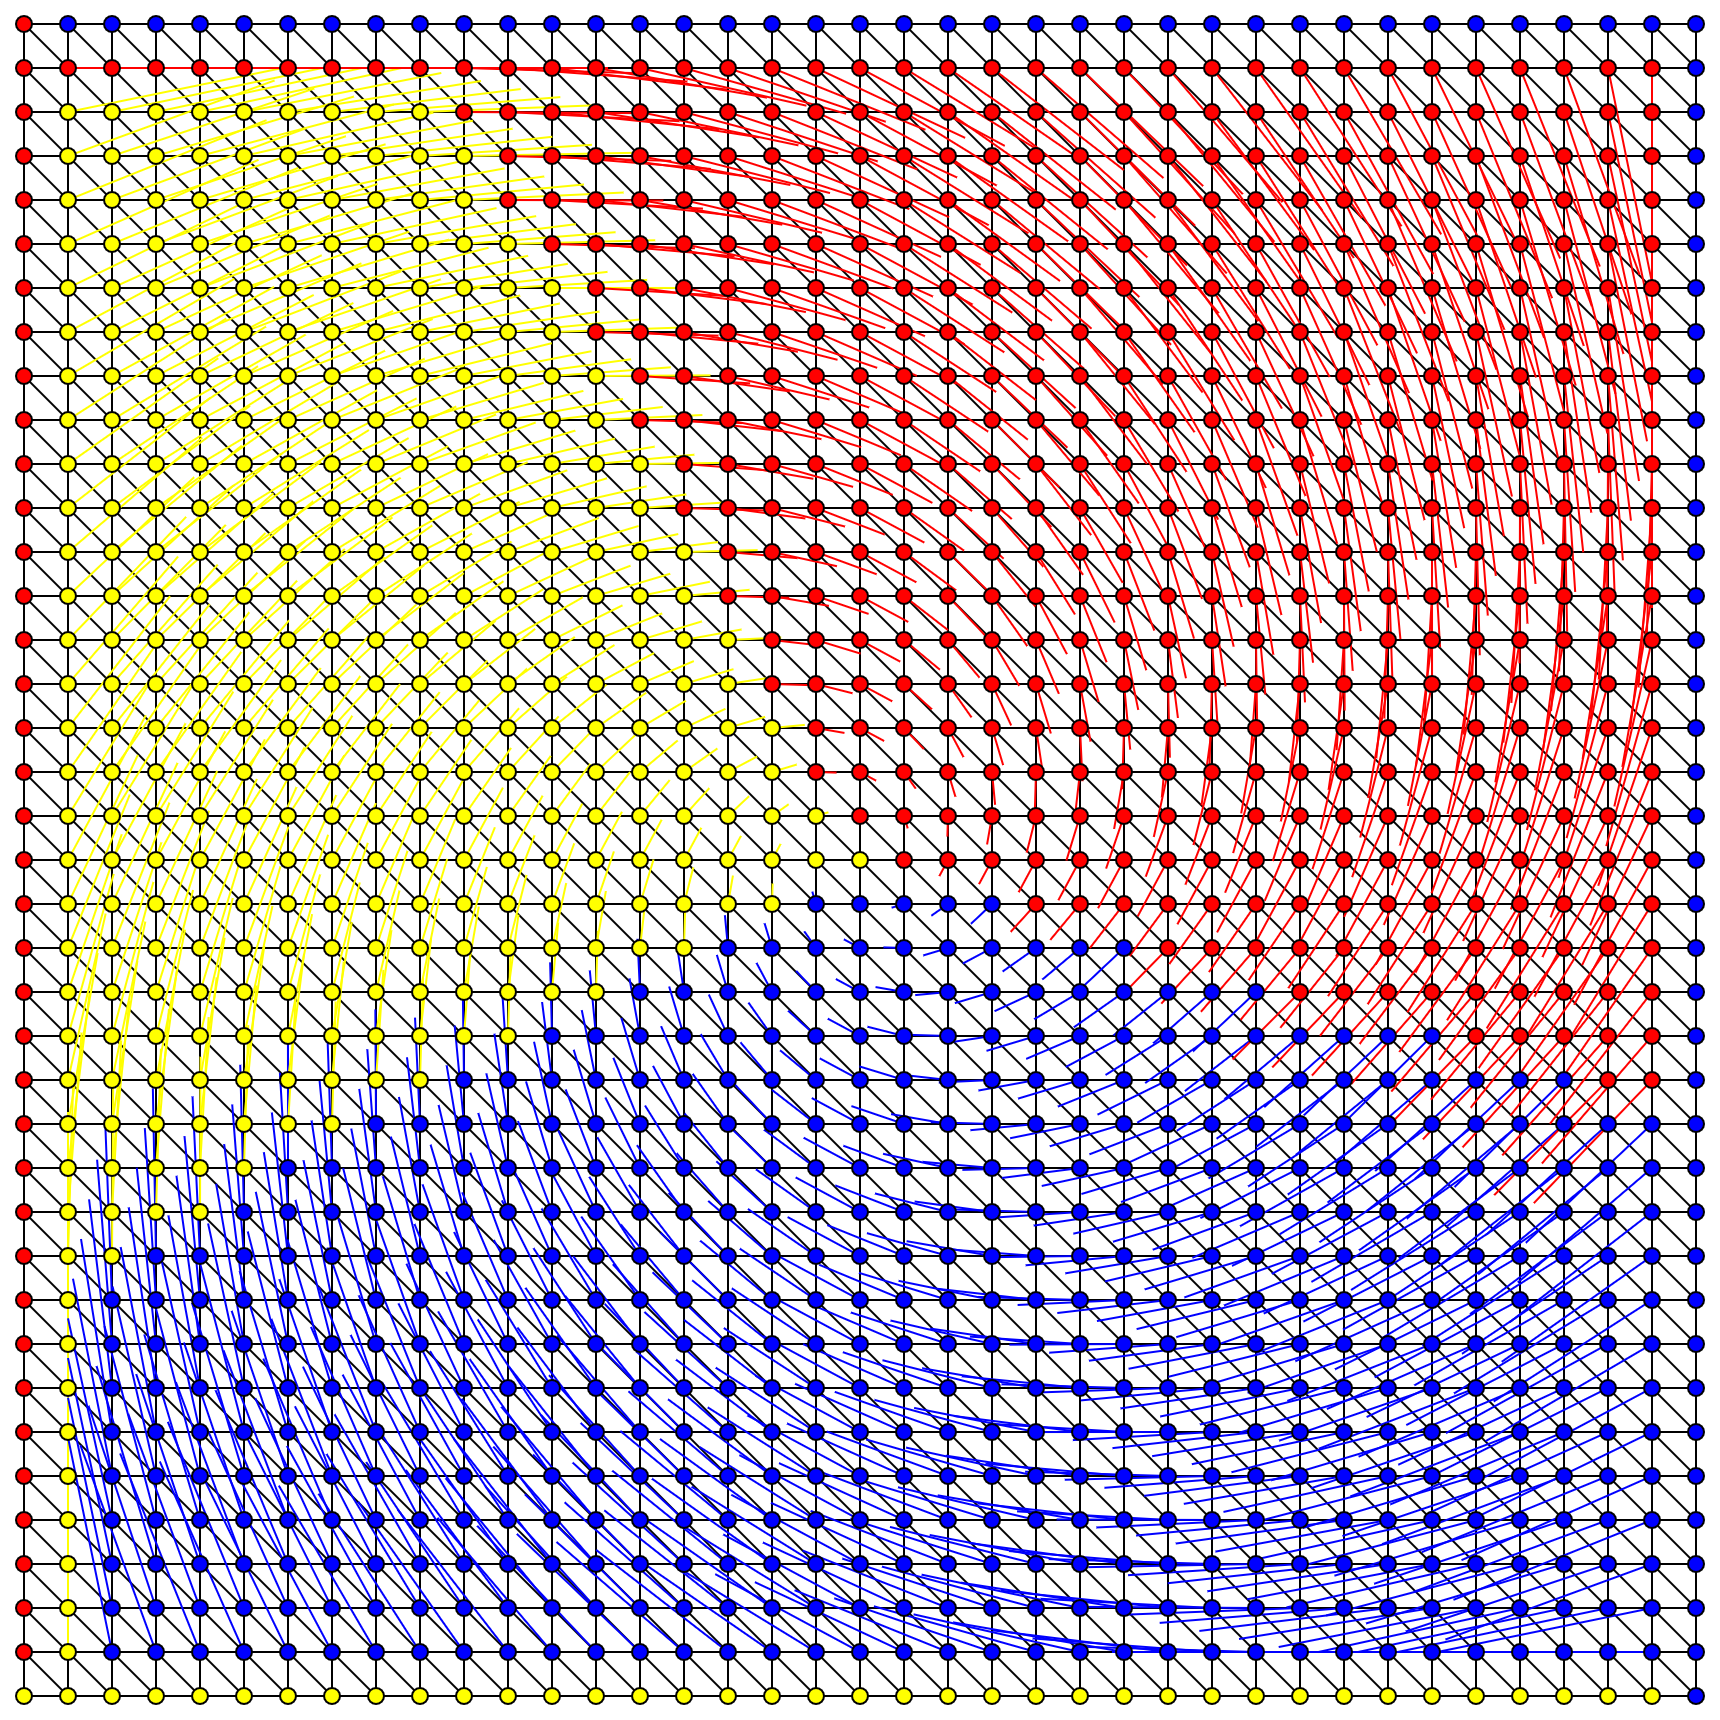
\includegraphics[width=0.9\textwidth]{ContractionToEOPL_example1_displacement}
  \end{figure}

  \begin{figure}[h]
    \caption{Potentials for a coarser discretization of the same spiral as above.}
    \centering
    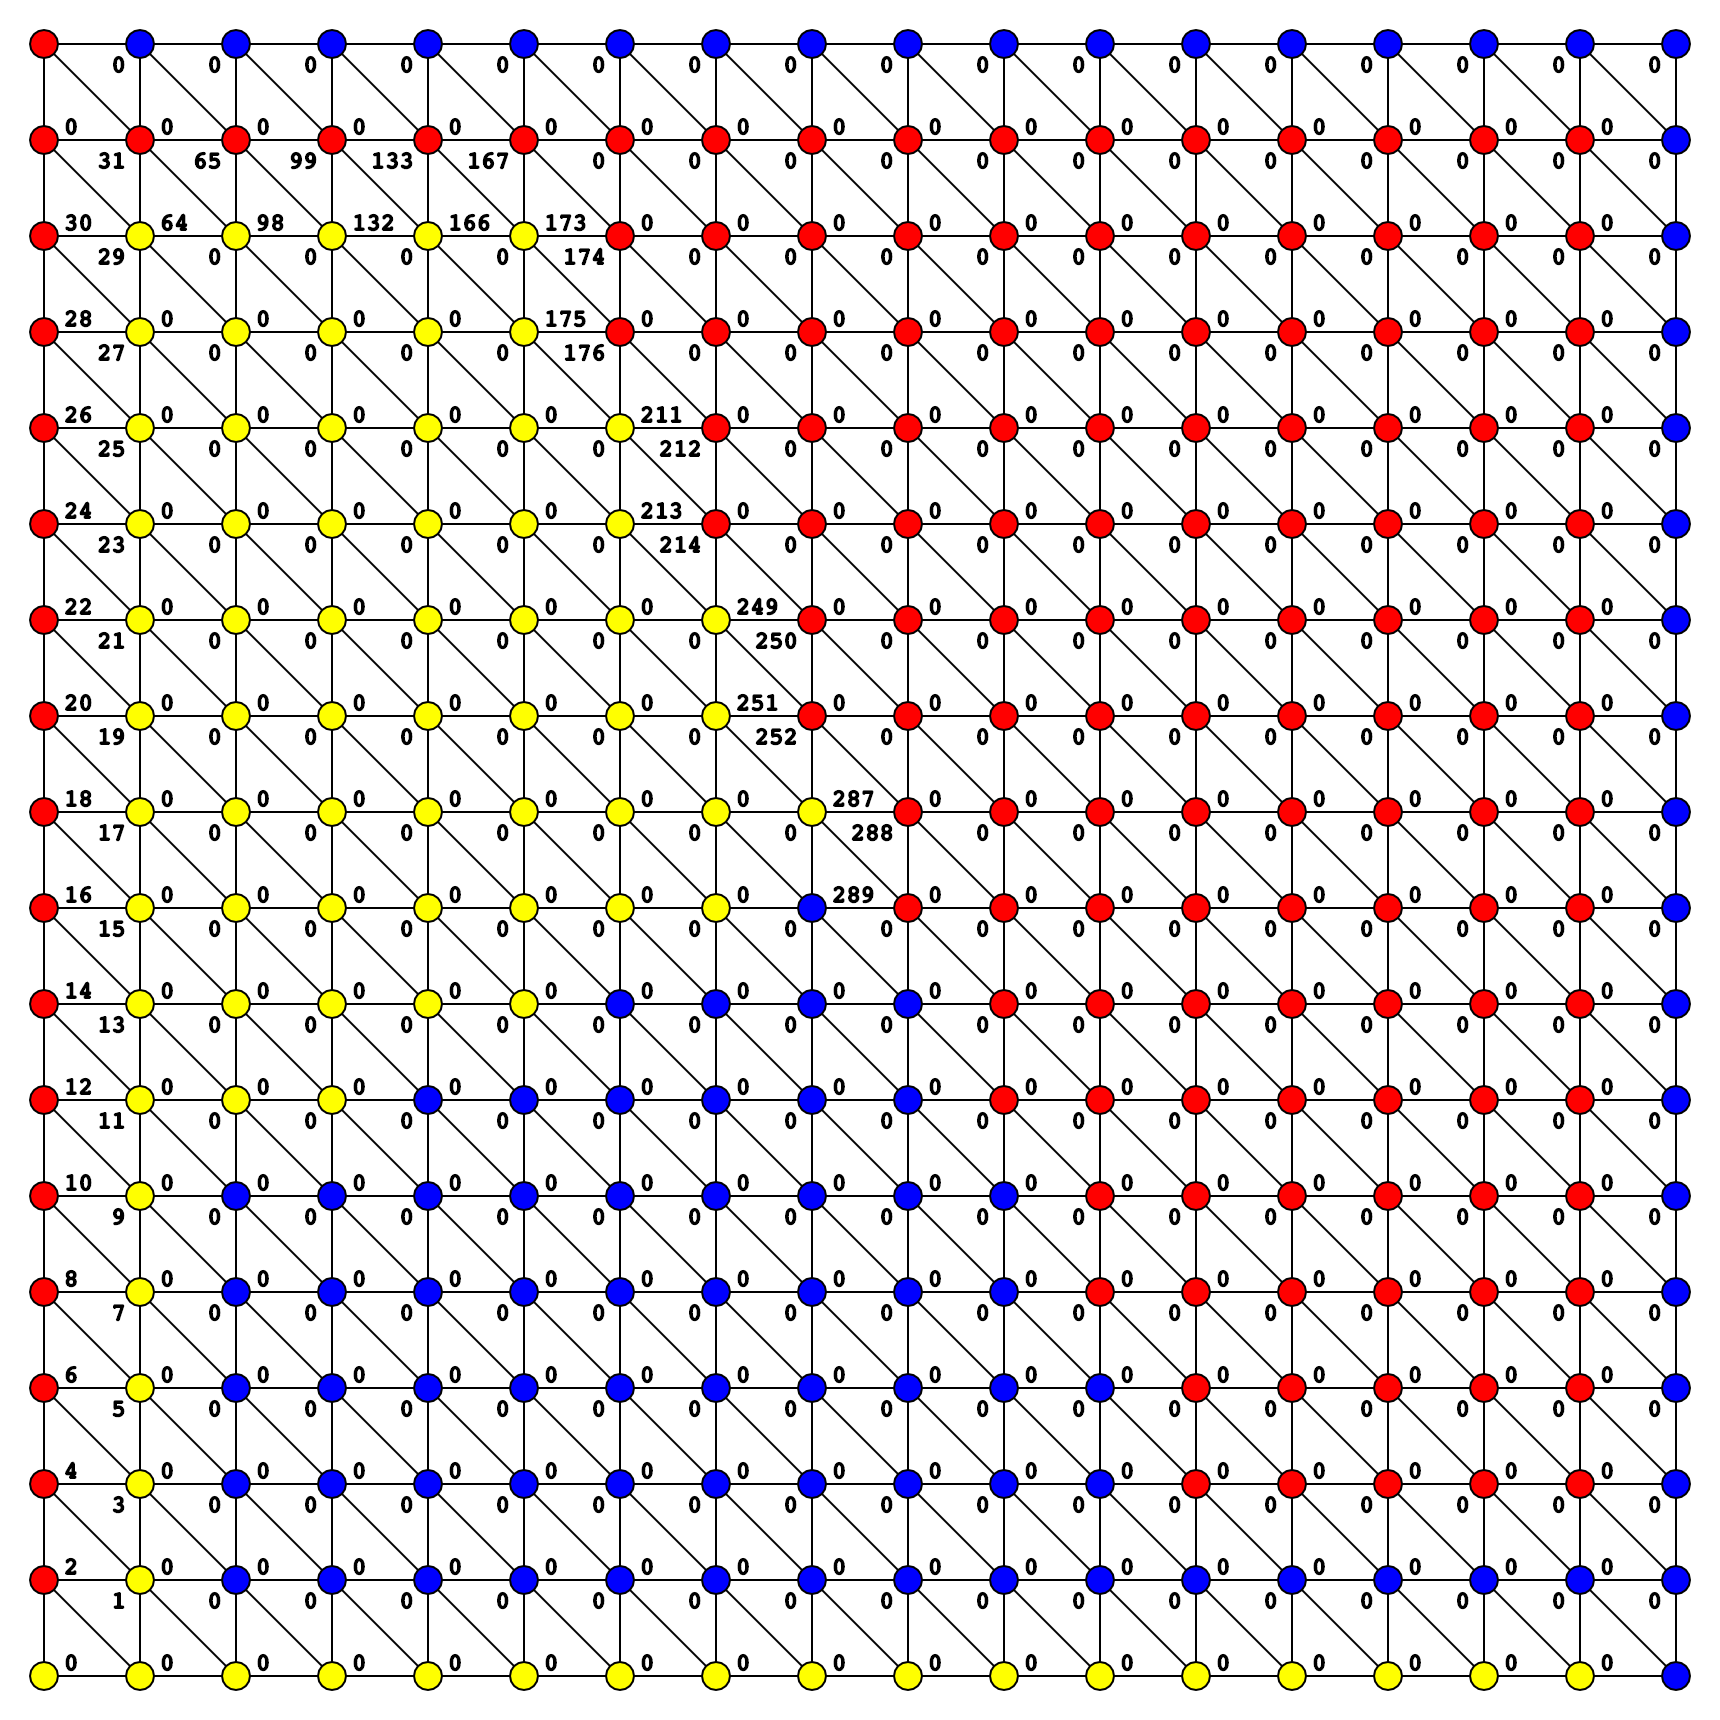
\includegraphics[width=0.9\textwidth]{ContractionToEOPL_example1_potentials}
  \end{figure}

  \begin{lemma} \label{lemma:PotentialsIncreaseAlongPaths}
    For any triangles $T_1,T_2 \in \Delta_D$, if $\Succ(T_1) = T_2$ and $\Pred(T_2) = T_1$, then $\Value(T_1) < \Value(T_2)$. 
  \end{lemma}

  \begin{proof}
    Since $T_1$ and $T_2$ are adjacent in the \EOPL graph, they must share a side. Furthermore, $T_2$ cannot be to the left of $T_1$ since any we break all paths rather than introduce an edge to the left. Thus, there are three cases to consider:
    \begin{description}
    \item[$T_2$ is above $T_1$] In this case, the potential at $T_2$ and $T_1$ will be computed counting from the bottom of the column, and $\Value(T_2) > \Value(T_1)$.
    \item[$T_2$ is below $T_1$] In this case, the potential at $T_2$ and $T_1$ will be computed counting from the top of the column and $\Value(T_2) > \Value(T_1)$. 
    \item[$T_2$ is to the right of $T_1$] The potential of any triangle (with non-zero potential) in a given column will be greater than the potential of any triangle in any column to the left of the given column. Thus, $\Value(T_2) > \Value(T_1)$.
    \end{description}
  \end{proof}

  \begin{lemma} \label{EndOfLineSolutions}
    Any solution $T \in \Delta_D$ of type \ref{A1} gives a solution for the \TwoDContractionMap instance.
  \end{lemma}
  \begin{proof}
     Consider a solution $T \in \Delta_D$ of type \ref{A1}. By construction, every triangle without a red-yellow side is in a self-loop, so $T$ must have at least one red vertex and at least one yellow vertex. There are two cases to consider: Either $T$ also has a blue vertex, in which it is a trichromatic triangle, and gives a solution of type \ref{B1} by Lemma \ref{lemma:TrichromaticTriangles}, or two of $T$'s vertices are either red or yellow. In the latter case, one of the red-yellow sides must not correspond to a valid edge in the graph, since $T$ is the either the start or end of a line. The only red-yellow sides that don't correpons to valid edges in the graph are those that are predecessor edges to the right, or successor edges to the left. In either of those case, there is a yellow vertex above a red vertex in $T$, and by Lemma \ref{lemma:YellowAboveRed}, the yellow and red vertices witness $f$ not being a contraction map, and give a solution of type \ref{B2}.
    \end{proof}
    
    To complete the reduction, we choose for our starting triangle the following: \[(-1/n,0),(0,-1/n),(-1/n,-1/n)\]
  
  \begin{enumerate}
  \item As far as I can tell, there can be edges pointing up in the graph other than those induced by the boundary. I should come up with an example containing edges of that sort. 
  \item I believe this can be generalized to \ThreeDContractionMap, since I think it will be the case that paths will be limited in a similar way, so that we can assign consistent potential values to each point. 
  \item We can look at the DTZ paper and see if their hardness proof gives us a metric from which we could do this same reduction. Or we could modify their metric somehow and still carry out the same sort of proof.
  Can we use the $\lambda$-Lipschitz continuity of $d$ in the DTZ definition of MetricBanach to generalize this argument to that definition. 

  If it's the case that we're given a metric which is of the form $d(x,y) = g(\Abs{x_1-x_2},\Abs{y_1-y_2})$, where $g$ is a non-decreasing function in both arguments, then I think everything works out. We may be able to extract solutions from violations of this. (Probably not, seems too rigid a constraint.)

  Fix the JavaScript to make sure all the colors are being computed correctly, and then update the images accordingly.

  \end{enumerate}

  One other interesting observation: When $f$ is in fact a contraction map, there can be at most one edge from left-to-right in any given column by Lemma \ref{lemma:YellowAboveRed}. 

  Can we go from EOPL to a standard norm-based contraction in $n$-dimensions?

  What is the role of uniqueness of solutions.
  